\subsubsection{Phase 1}
\label{subsub:phaseone}
In this phase we transform every $q_i \in Q$ to sequences of game blocks. These sequences will be part of the block states $P_1, \ldots P_n$ in the game $\mathcal{G}$ of the constructed \textit{k-cleared-cells} instance. The transformation is done by creating a sequence of 1 $\mathbf{H}_{H}$, $q_i$ $\mathbf{H}$ and 1 $\mathbf{H}_H$ blocks (in their initial state) for each given $q_i$.

\begin{figure}[H]
    \centering
    \resizebox{0.4\textwidth}{!}{
    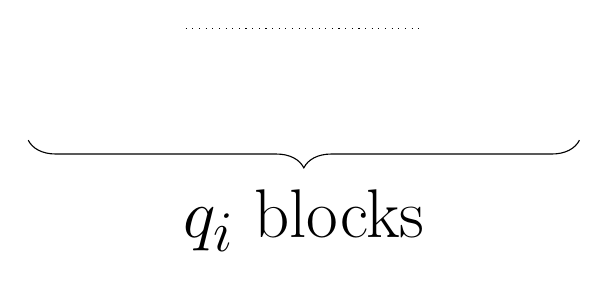
\begin{tikzpicture}
        \startb{0}{0}
        \middleb{3}{0}
        \draw[dotted] (5, 1) -- (8, 1);
        \middleb{8}{0}
        \startb{11}{0}
        \draw [decorate,decoration={brace,amplitude=10pt,mirror},xshift=0pt,yshift=-12pt]
        (3, 0) -- (10, 0) node [below,black,midway,yshift=-0.5cm]
        {\Huge $q_i$ blocks};
    \end{tikzpicture}
    }
    \caption{Transformation of \textit{Subset sum} element $q_i$}
    \label{fig:transforms}
\end{figure}

When placing the first block it is evident that we have only two possibilities. Either we place the $\mathbf{H}_H$ block in column 2-3 of  well 1, or in the respective columns of well 2. This transforms the chosen well from a closed to an open state. We then proceed to placing the middle $q_i$ blocks. When deciding the outcome of these placements the following lemmas are of use:\\

\begin{lem}
\label{lem:permclose}
In phase 1, placing a $\mathbf{H}$ block in any other column than 4-5 in any well will make the same well blocked.
\end{lem}

\begin{proof}
In the first case, the well is closed. We can only place the $\mathbf{H}$ block in column 2-3. Since no cells are cleared as a result, column 1 to 4 are filled except for the top two rows. We therefore cannot place any block in these columns without a game over. Either the column right of column 5 is filled, or the gameboard has ended. Since column 4 is also filled, we cannot place any block in column 5. Thus the well is permanently closed.

In the second case, the well is open. Apart from column 4-5, the $\mathbf{H}$ block can only be placed in column 3-4. This does not clear any cells as a result. Thus with the same arguments as in the first case, the well is blocked.
\end{proof}

Since later in the proof it will become apparent that having a blocked well makes it impossible to construct a optimal trajectory sequence, lemma~\ref{lem:permclose} leaves us no choice but to place all $\mathbf{H}$ blocks in column 4-5 of the open well. Finally the last $\mathbf{H}_H$ block must be placed either in column 2-3 of a closed well, or column 3-4 of an open well, in order to not block a well.

\bigbreak

\begin{lem}
In phase 1, for each well: Column 1 is unchanged from $B_0$. Column 2-4 will be filled below row $2 \left( \sum Q + K + 1 \right) - 3$. Column 5 is empty as long as the well is not blocked.
\end{lem}

\begin{proof}
The following holds for each column:

Column 1 is initially filled completely with alternating rows except the two top rows that would result in an instant losing state. From lemma \ref{lem:alternatingrows} it is known that a column with an interval of alternating rows may only clear the bottom or top cell in the interval. Thus it is impossible to clear any cell in the column without putting the game in a losing state. 

Column 2 is initially filled beneath row $2 \left( \sum Q + K + 1 \right) - 3$ with alternating rows. Because column 2 has alternating rows there is no way to clear rows from anywhere except the top of the column. It is known that column 1 can not be cleared which leaves two requirements to clear any of the cells and lower the height of column 2. Column 3 must leave place for a white cell at $2 \left( \sum Q + K + 1 \right) - 4$ and a fitting block must be dropped to create a white $2 \times 2$ block. Both of these requirements are unfulfilled but we will only prove the first requirement.

Let $I$ be the interval:
\begin{equation*}
\left[ 2 \left( K - 1 \right) + 1, 2 \left( \sum Q + K + 1 \right) - 4 \right]
\end{equation*}

Column 3 is initially filled beneath row $2 \left( \sum Q + K + 1 \right) - 3$. The interval $I$ consists of alternating rows. Beneath row $2 \left( K - 1 \right) + 1$ the column is filled with white cells. In a closed well rows in column 3 can only be cleared if column 2 leaves place for a black cell and a fitting block is dropped. However it is already known that column 2 can not clear any rows if there have not been any cleared rows in column 3. The only other way column 3 can clear rows and lower its height is by clearing rows beneath $2 \left( K - 1 \right) + 1$. For this to happen there must be white cells in column 4 beneath row $2 \left( K - 1 \right) + 1$.

Column 4 is initially filled beneath row $2 \left( \sum Q + K + 1 \right) - 3$ with black cells. To clear rows in column 4 and lower its height we need need two adjacent rows with black cells in either column 3 or column 5 somewhere beneath the same row. For this to happen in column 3, the height of column 3 needs to be reduced with at least two rows. It is known that this can only happen if there are white cells beneath row $2 \left( \sum Q + K + 1 \right) - 3$ in column 4. Thus the only way to clear rows and lower column 4's height is to have two adjecent rows in column 5 with black cells beneath row $2 \left( \sum Q + K + 1 \right) - 3$.

Column 5 is initially empty. The lemma says that the column is empty as long as the well is not blocked. When the well is closed there is no way to fill any cells in the column. When the well is open we can drop half a block down column 5 by placing the given block on column 4-5. The two blocks the player can place is $\mathbf{H}$ and $\mathbf{H}_H$. Placing a $\mathbf{H}_H$ block fills column 5 but also blocks the well. Placing a $\mathbf{H}$ block will create a black block that clears the cells in column 5 and the two bottom most cells in column 4. Two white cells are placed on top of column 4 when placing the block and column 4 will therefore not lower its height unless the white cells in column 4 are cleared together with the white cells in column 3. This happens if the player places $\sum Q + 1$ $\mathbf{H}$ blocks. However the amount of $\mathbf{H}$ given during phase 1 is $\sum Q$ and will therefore not happen. For there to be any filled cells in column 5 without blocking the well the player need to place $\sum Q + K$ blocks in column 4-5 which is not possible for the same reason.

Thus all parts of the lemma holds.
\end{proof}

\begin{figure}[H]
    \centering
    \begin{subfigure}[b]{0.55\textwidth}
        \resizebox{\linewidth}{!}{
            \begin{tikzpicture}
                \welldefault{0}{0}
                \startb{1}{10}
                \welldefault{5}{0}
                \draw[dashed] (0, 0) -- (0, 12);
                \draw[dashed] (10, 0) -- (10, 12);
                \draw[dashed] (0, 0) -- (10, 0);
                \draw[->, line width=10pt] (11, 6) -- (14, 6);
                \wellopenwhole{15}{0}
                \welldefault{20}{0}
                \draw[dashed] (15, 0) -- (15, 12);
                \draw[dashed] (25, 0) -- (25, 12);
                \draw[dashed] (15, 0) -- (25, 0);
            \end{tikzpicture}
        }
        \caption{First block}
        \vspace*{0.5cm}
    \end{subfigure}

    \begin{subfigure}[b]{0.55\textwidth}
        \resizebox{\linewidth}{!}{
            \begin{tikzpicture}
                \wellopenwhole{0}{0}
                \middleb{3}{10}
                \welldefault{5}{0}
                \draw[dashed] (0, 0) -- (0, 12);
                \draw[dashed] (10, 0) -- (10, 12);
                \draw[dashed] (0, 0) -- (10, 0);
                \draw[->, line width=10pt] (11, 6) -- (14, 6);
                \wellopenwhole{15}{0}
                \cellw{18}{7}
                \cellw{18}{6}
                \welldefault{20}{0}
                \draw[dashed] (15, 0) -- (15, 12);
                \draw[dashed] (25, 0) -- (25, 12);
                \draw[dashed] (15, 0) -- (25, 0);
            \end{tikzpicture}
        }
        \caption{Middle blocks}
        \vspace*{0.5cm}
    \end{subfigure}

    \begin{subfigure}[b]{0.55\textwidth}
        \resizebox{\linewidth}{!}{
            \begin{tikzpicture}
                \wellopenwhole{0}{0}
                \cellw{3}{7}
                \cellw{3}{6}
                \startb{2}{10}
                \welldefault{5}{0}
                \draw[dashed] (0, 0) -- (0, 12);
                \draw[dashed] (10, 0) -- (10, 12);
                \draw[dashed] (0, 0) -- (10, 0);
                \node at (12.5, 6)
                {\Huge or};
                \wellopenwhole{15}{0}
                \cellw{18}{7}
                \cellw{18}{6}
                \welldefault{20}{0}
                \startb{21}{10}
                \draw[dashed] (15, 0) -- (15, 12);
                \draw[dashed] (25, 0) -- (25, 12);
                \draw[dashed] (15, 0) -- (25, 0);
            \end{tikzpicture}
        }
        \caption{Final block}
    \end{subfigure}

    \caption{Block placement in phase 1}
    \label{fig:placement}
\end{figure}

Assuming that no blocks has been placed such that any well is blocked, the following invariants holds at the start of the sequence corresponding to $q_i$:

\begin{enumerate}
\item Either both of the wells are closed, or both of the wells are open.

\item Column 1, 3 and 5 in any well are unchanged from the initial gameboard. Column 2 is unchanged except from the top two rows (which may be black or empty).

\item Let $q_0 = 0$. This does not change the semantics of the given \textit{Subset sum} instance. Then in total 
\begin{equation*}
    2 \left( i-1 \right) + \sum_{j=0}^{i-1} q_j
\end{equation*}
blocks have been placed.

\item Since each block placement clears exactly 4 cells
\begin{equation*}
    8 \left( i-1 \right) + 4 \sum_{j=0}^{i-1} q_j
\end{equation*}
cells have been cleared.

\item There exists: 
    \begin{equation*}
        M_1, M_2 \subseteq \{q_0, \ldots q_{i-1}\}, M_1 \cap M_2 = \varnothing, M_1 \cup M_2 = \{q_0, \ldots, q_{i-1}\}
    \end{equation*}
such that for any well $w \in \{1,2\}$ it holds that the rows in interval
    \begin{equation*}
        \left[ 2 \left( K-1 + \sum Q - \sum M_w \right) +1, 2 \left( K-1 + \sum Q \right) \right]
    \end{equation*}
consists of white cells in column 4, and the rows in interval
    \begin{equation*}
        \left[ 1, 2 \left( K-1 + \sum Q - \sum M_w \right) \right]
    \end{equation*}
consists of black cells in column 4.
\end{enumerate}

\begin{figure}[H]
    \centering
    \resizebox{!}{0.3\paperheight}{
    \begin{tikzpicture}
        \invariantchart{0}{0}
        \draw[dashed] (-1, 0) -- (6, 0);
        \draw[dashed] (-1, 6) -- (6, 6);
        \draw[dashed] (-1, 12) -- (6, 12);
        \draw[dashed] (-1, 20) -- (6, 20);
        \draw[dashed] (5, 0) -- (5, 22);
        \node at (0.5, -0.5) {\large 1};
        \node at (1.5, -0.5) {\large 2};
        \node at (2.5, -0.5) {\large 3};
        \node at (3.5, -0.5) {\large 4};
        \node at (4.5, -0.5) {\large 5};
        \draw [decorate,decoration={brace,amplitude=10pt},xshift=-12pt,yshift=0pt]
        (0, 0) -- (0, 6) node [left,align=right,black,midway,xshift=-1cm]
        {\huge $2 \left( K-1 \right)$ rows};
        \draw [decorate,decoration={brace,amplitude=10pt},xshift=-12pt,yshift=0pt]
        (0, 6) -- (0, 12) node [left,align=right,black,midway,xshift=-1cm]
        {\huge $2 \left( \sum Q - \sum M_w \right)$ rows};
        \draw [decorate,decoration={brace,amplitude=10pt},xshift=-12pt,yshift=0pt]
        (0, 12) -- (0, 20) node [left,align=right,black,midway,xshift=-1cm]
        {\huge $2 \sum M_w $ rows};
        \draw (3.5, 0.5) -- (7, 0.5) node [right, black, xshift=1cm] 
        {\huge row 1};
        \draw (3.5, 5.5) -- (7, 5.5) node [right, black, xshift=1cm, yshift=-0.5cm] 
        {\huge row $2 \left( K-1 \right)$};
        \draw (3.5, 6.5) -- (7, 6.5) node [right, black, xshift=1cm, yshift=0.5cm] 
        {\huge row $2 \left( K-1 \right) + 1$};
        \draw (3.5, 11.5) -- (7, 11.5) node [right, black, xshift=1cm, yshift=-0.5cm] 
        {\huge row $2 \left( K-1 + \sum Q - \sum M_w \right)$};
        \draw (3.5, 12.5) -- (7, 12.5) node [right, black, xshift=1cm, yshift=0.5cm] 
        {\huge row $2 \left( K-1 + \sum Q - \sum M_w \right) +1$};
        \draw (3.5, 19.5) -- (7, 19.5) node [right, black, xshift=1cm] 
        {\huge row $2 \left( \sum Q + K - 1 \right)$};
    \end{tikzpicture}
    }
    \caption{Depiction of invariants}
    \label{fig:invariant}
\end{figure}

When every block sequence corresponding to the elements of $Q$ has been placed, $a$ elements has been transformed. For all purposes of this proof this is equivalent to being at the start of the sequence corresponding to element $q_{a+1}$, even though strictly speaking no such element is given. Thus we can assume $i = a+1$ and from the invariants we obtain:

\begin{enumerate}
\item Still holds.
\item Still holds.
\item In total
\begin{equation*}
    2a + \sum Q
\end{equation*}
blocks have been placed.

\item In total
\begin{equation*}
    8a + 4 \sum Q
\end{equation*}
cells have been cleared.

\item There exists:
\begin{equation*}
    M_1, M_2 \subseteq Q, M_1 \cap M_2 = \varnothing, M_1 \cup M_2 = Q
\end{equation*}
such that for any well $w \in \{1,2\}$ it holds that the rows in interval
\begin{equation*}
        \left[ 2 \left( K-1 + \sum Q - \sum M_w \right) +1, 2 \left( K-1 + \sum Q \right) \right]
    \end{equation*}
consists of white cells in column 4, and the rows in interval
    \begin{equation*}
        \left[ 1, 2 \left( K-1 + \sum Q - \sum M_w \right) \right]
    \end{equation*}
consists of black cells in column 4.

\end{enumerate}

Thus at most $8a + 4 \sum Q$ cells have been cleared at the end of this phase.
